\documentclass{article}

%%%%%%% PACKAGES %%%%%%%%
\usepackage[utf8]{inputenc}
\usepackage[margin=2cm]{geometry}
\usepackage{import}
\usepackage{blindtext}
\usepackage{setspace}
\usepackage{listings}
\usepackage[usenames,dvipsnames,table]{xcolor}
\usepackage{graphicx}
\usepackage{adjustbox}
\usepackage{stackengine}[2013-10-15]
\newcommand\textss[1]{\stackengine{.9ex}{}{\scriptsize#1}{O}{l}{F}{F}{L}}
\graphicspath{ {./images/} }
\usepackage{notoccite}
\usepackage{lscape}
\usepackage{caption}
\usepackage{csvsimple}
\usepackage{hyperref}
\usepackage{lipsum}
\usepackage{xcolor}

\colorlet{punct}{red!60!black}
\definecolor{background}{HTML}{EEEEEE}
\definecolor{delim}{RGB}{20,105,176}
\colorlet{numb}{magenta!60!black}
\lstdefinelanguage{json}{
    basicstyle=\normalfont\ttfamily,
    numbers=left,
    numberstyle=\scriptsize,
    stepnumber=0,
    numbersep=8pt,
    showstringspaces=false,
    breaklines=true,
    frame=lines,
    backgroundcolor=\color{background},
    literate=
     *{0}{{{\color{numb}0}}}{1}
      {1}{{{\color{numb}1}}}{1}
      {2}{{{\color{numb}2}}}{1}
      {3}{{{\color{numb}3}}}{1}
      {4}{{{\color{numb}4}}}{1}
      {5}{{{\color{numb}5}}}{1}
      {6}{{{\color{numb}6}}}{1}
      {7}{{{\color{numb}7}}}{1}
      {8}{{{\color{numb}8}}}{1}
      {9}{{{\color{numb}9}}}{1}
      {:}{{{\color{punct}{:}}}}{1}
      {,}{{{\color{punct}{,}}}}{1}
      {\{}{{{\color{delim}{\{}}}}{1}
      {\}}{{{\color{delim}{\}}}}}{1}
      {[}{{{\color{delim}{[}}}}{1}
      {]}{{{\color{delim}{]}}}}{1},
}

\newcommand\blfootnote[1]{%
  \begingroup
  \renewcommand\thefootnote{}\footnote{#1}%
  \addtocounter{footnote}{-1}%
  \endgroup
}

\usepackage{acro}

\DeclareAcronym{bdd}{
  short = BDD,
  long = Behaviour-Driven Development,
  class = B
}

\DeclareAcronym{ci}{
  short = CI,
  long = Customer Interruption,
  class = B
}

\DeclareAcronym{da}{
  short = DA,
  long = Distribution Automation,
  class = B
}

\DeclareAcronym{flisr}{
  short = FLISR,
  long = {Fault Location, Isolation and Service Restoration},
  class = B
}

\DeclareAcronym{ict}{
  short = ICT,
  long = Information and Communication Technology,
  class = B
}

\DeclareAcronym{igsd}{
  short = IGSD,
  long = Intelligent Grid Switching Devices,
  class = B
}

\DeclareAcronym{iot}{
  short = IoT,
  long = Internet of Things,
  class = B
}

\DeclareAcronym{kpi}{
  short = KPI,
  long = Key Performance Indicator,
  class = B
}

\DeclareAcronym{mas}{
  short = MAS,
  long = Multi Agent Approach,
  class = B
}

\usepackage[acronym]{glossaries}
\makenoidxglossaries
\newglossaryentry{adms}
{
    name=Advanced Distribution Management System (ADMS),
    description={A software platform containing a suite of functions to support distribution network management and optimisation}
}

\newglossaryentry{cml}
{
    name=Customer Minutes Lost (CML),
    description={Measurement of the duration of interruption of supply over the course of a year. Consists of the average CML per consumer per year, in the event a supply interruption lasts up to or more than 3 minutes}
}

\newglossaryentry{dso}
{
    name=Distribution System Operator (DSO),
    description={Designated entity responsible for management of the distribution network from source of generation to final consumer}
}

\newglossaryentry{fpi}
{
    name=Fault Passage Indicator (FPI),
    description={Indicator notifying that an on-pole switch has detected a fault on its specific point of the network}
}

\newglossaryentry{gis}
{
    name=Geographical Information System (GIS),
    description={Software system utilised to analyse and visualise data containing geographic information}
}

\newglossaryentry{lbfm}
{
    name=Load Break Fault Make Switch (LBFM),
    description={On-pole circuit breaker which can be controlled to energise or de-energise a section of network in the event of over-load, fault event or required maintenance}
}

\newglossaryentry{lvi}
{
    name=Loss of Voltage Indicator (LVI),
    description={Indicator notifying that an on-pole switch has lost supply on its specific point of the network}
}


\newglossaryentry{lv}
{
    name=Low Voltage (LV) Network,
    description={Distribution network which transmits to end customers, generally at mains rated voltage (230V single phase \& 400V 3 phase for the Irish LV network)}
}

\newglossaryentry{mv}
{
    name=Medium Voltage (MV) Network,
    description={Distribution network which transmits at voltages above 1kV (kilovolt) (10kV, 20kV \& 38kV for the Irish MV network)}
}

\hypersetup{
    colorlinks=true,
    linkcolor=black,
    citecolor=black,
    filecolor=magenta,
    urlcolor=cyan
    }

\urlstyle{same}
\onehalfspace

\title{\huge{\textbf{Dissertation}} \\
\LARGE{A Distributed Edge FLISR Solution \& Network Simulation Test Platform}}
\author{Darren Leniston \\
        Supervisor - Dr Kieran Murphy
}
\date{September 2023}

% Allow rowstyles to be set
\newcolumntype{$}{>{\global\let\currentrowstyle\relax}}
\newcolumntype{^}{>{\currentrowstyle}}
\newcommand{\rowstyle}[1]{\gdef\currentrowstyle{#1}%
  #1\ignorespaces
}
% Table style
\newcommand{\header}{\rowcolor{tableHeading}\rowstyle{\bfseries}}
\newcommand{\row}{\rowstyle{\normalsize{}}}
\newenvironment{tabledata}[1][1]{%
  \renewcommand*{\extrarowheight}{0.1cm}%
  \tabular%
}{%
  \endtabular
}
\rowcolors{2}{tableShading}{white}
%Default table position
\makeatletter
\def\fps@table{htbp}
\makeatother
\definecolor{tableHeading}{HTML}{c2c9d4}
\definecolor{tableShading}{HTML}{e8eaef}
\begin{document}
\pagenumbering{roman}
\clearpage\maketitle
\thispagestyle{empty}
\begin{center}
    \begin{figure}[h]
        \centering
        
\includegraphics[width=8cm]{SETU}
        \label{fig:logo}
    \end{figure}
    \large{MSc in Computing (Enterprise Software Systems) \\
    School of Science and Computing}
\end{center}
\newpage
\import{parts/}{abstract.tex}
\newpage
\import{parts/}{declaration.tex}
\newpage
\setcounter{page}{1}
\tableofcontents
\listoffigures
\listoftables

\glsaddallunused
\printnoidxglossaries
\printacronyms[include-classes=B,name=List of Acronyms]
\newpage
\pagenumbering{arabic}
\import{parts/1_introduction/}{introduction.tex}
\import{parts/2_literature/}{literature.tex}
\import{parts/3_methods/}{methods.tex}
\import{parts/4_results/}{results.tex}
\import{parts/5_conclusion/}{conclusion.tex}
\import{parts/6_exploitation/}{exploitation.tex}
\clearpage
\bibliographystyle{plain}
\bibliography{references/references}
\clearpage

\appendix
\section{Appendices}
\label{sec:appendices}
\subsubsection{FLISR Edge simulation platform user stories}
\label{sec:appendix_a}

\begin{figure}[h]
  \centering
  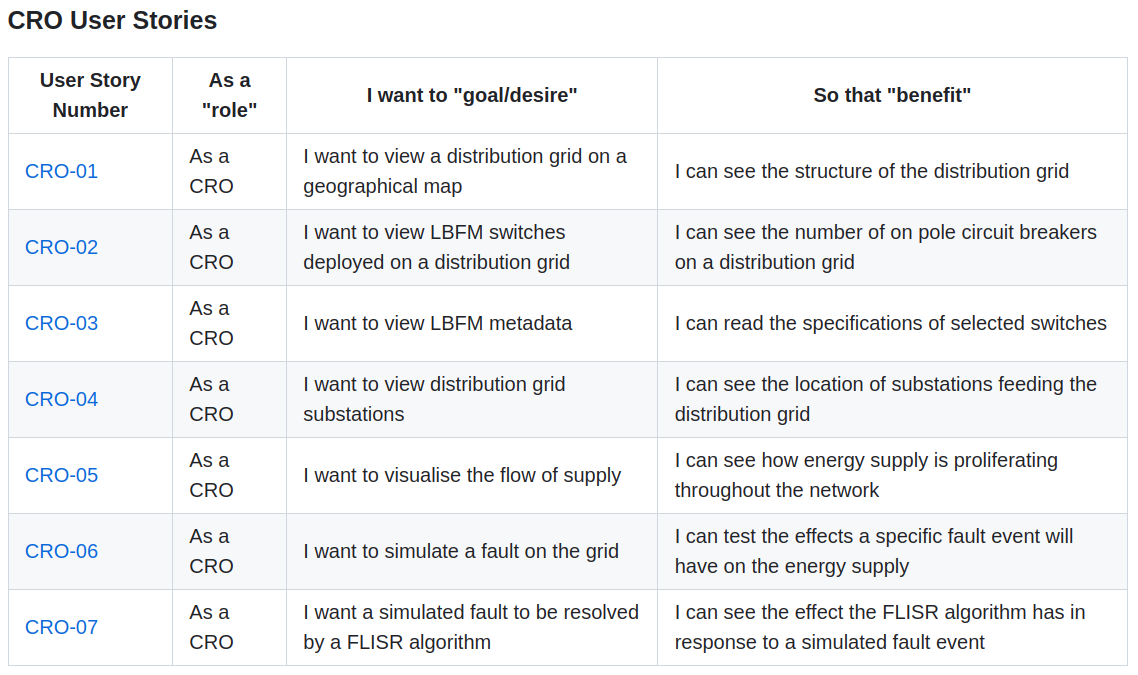
\includegraphics[width=0.8\textwidth]{fig_cro}
\end{figure}

\begin{figure}[h]
  \centering
  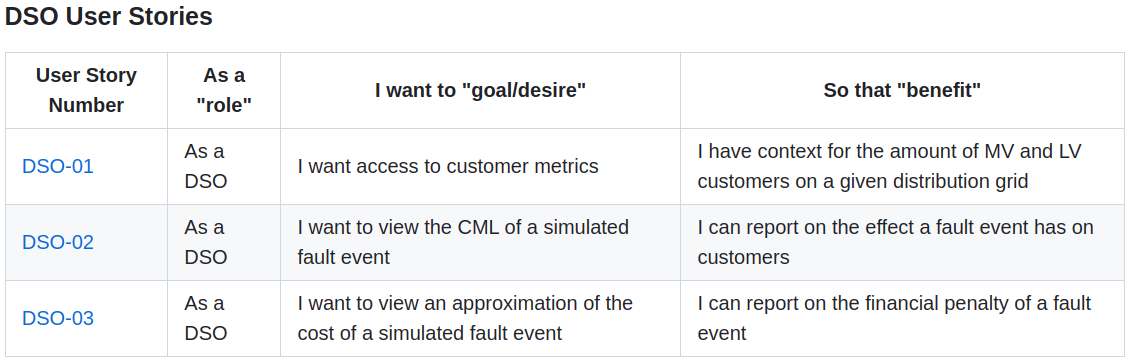
\includegraphics[width=0.8\textwidth]{fig_dso}
\end{figure}

% subsection appendix_a (end)

\clearpage
\subsubsection{FLISR Edge user stories}
\label{sec:appendix_b}

\begin{table}
\hrule height 0.1cm  \vspace{0.5cm}
  \caption{\label{table:ap_3}FLISR Master user stories}
  \centering
  \begin{adjustbox}{width=\textwidth}
  \begin{tabular}{|l|l|l|l|p{5cm}}
  \hline
    \header User story number & As a "role" & I want to "goal/desire" & So that "benefit" \\ [0.1cm]
    \row  FM-01 & As a FLISR Master & I want to have a central view of the distribution grid & \parbox{8cm}{I can see the structure of the distribution grid} \\ [0.5cm]
    \row  FM-02 & As a FLISR Master & I to have a central FLISR algorithm & \parbox{8cm}{I can resolve faults from a central location} \\ [0.5cm]
    \row  FM-03 & As a FLISR Master & I want a view of edge devices & \parbox{8cm}{I can monitor edge devices installed on the grid} \\ [0.5cm]
    \row  FM-04 & As a FLISR Master & I want the ability to provision a network topology subset & \parbox{8cm}{FLISR nodes have a subset of the network related to them available} \\ [0.5cm]
    \row  FM-05 & As a FLISR Master & I want to provision a distributed FLISR algorithm & \parbox{8cm}{FLISR nodes have a subset of the FLISR algorithm} \\ [0.5cm]
    \row  FM-06 & As a FLISR Master & I want to recieve a heartbeat from FLISR nodes & \parbox{8cm}{I can monitor the connection of FLISR nodes on the grid} \\ [0.5cm]
    \row  FM-07 & As a FLISR Master & I want to recieve the status of LBFM switches from FLISR nodes & \parbox{8cm}{I know when a fault event occurs} \\ [0.5cm]
    \row  FM-08 & As a FLISR Master & I want to send commands to FLISR Nodes & \parbox{8cm}{I can action on fault restoration steps} \\ [0.5cm]
  \hline
  \end{tabular}
  \end{adjustbox}
\end{table}

\begin{table}
\hrule height 0.1cm  \vspace{0.5cm}
  \caption{\label{table:ap_4}FLISR Node user stories}
  \centering
  \begin{adjustbox}{width=\textwidth}
  \begin{tabular}{|l|l|l|l|p{5cm}}
  \hline
    \header User story number & As a "role" & I want to "goal/desire" & So that "benefit" \\ [0.1cm]
    \row  FN-01 & As a FLISR Node & I want to have a subset of the network topology & \parbox{8cm}{I can see the structure of the line on which I am located} \\ [0.5cm]
    \row  FN-02 & As a FLISR Node & I want to have a subset of the FLISR algorithm & \parbox{8cm}{I can resolve a fault event} \\ [0.5cm]
    \row  FN-03 & As a FLISR Node & I want to monitor the status of a switch & \parbox{8cm}{I can detect FPI and/or LVI} \\ [0.5cm]
    \row  FN-04 & As a FLISR Node & I want to sent a switches status to the FLISR Master & \parbox{8cm}{In the event of a fault the status of the switch is sent to the FLISR Master to process} \\ [0.5cm]
    \row  FN-05 & As a FLISR Node & I want to send a heartbeat to the FLISR Master & \parbox{8cm}{I can determine if communication is available} \\ [0.5cm]
    \row  FN-06 & As a FLISR Node & I want to act independently if communication with the FLISR Master is not available & \parbox{8cm}{I can use the subset of the FLISR algorithm to operate a switch if communication is not possible} \\ [0.5cm]
  \hline
  \end{tabular}
  \end{adjustbox}
\end{table}

% subsection appendix_b (end)

\clearpage
\subsubsection{FLISR Edge algorithms results sample}
\label{sec:appendix_c}

\begin{table}
\vspace{0.5cm}
    \centering
    \caption{\label{table:4}Centralised FLISR algorithm results sample}
    \begin{adjustbox}{width=\textwidth}
    \begin{tabular}{|l|l|l|l|l|l|l|l|l|p{5cm}}
    \hline
        start time & end time & faulted devices & down devices & operation & \parbox{2cm}{affected customers pre operation} & \parbox{2cm}{affected customers post operation} & \parbox{2cm}{cml per hour pre operation} & \parbox{2cm}{cml per hour post operation} \\ [0.1cm]
        2023-09-02 13:18:45.519 & 2023-09-02 13:18:45.726 & ['S507'] & \parbox{3cm}{"['S508', 'R518', 'S509', 'S697']"} & \parbox{5cm}{"S507 opened, S508 closed, R518 closed, S509 closed, S697 N/O point closed, "} & 1370 & 0 & 78090 & 0 \\ [0.5cm]
        2023-09-02 13:27:35.724 & 2023-09-02 13:27:35.916 & ['S507', 'S508'] & \parbox{3cm}{"['R518', 'S509', 'S697']"} & \parbox{5cm}{S507 opened, S508 opened, R518 closed, S509 closed, S697 N/O point closed, } & 1370 & 171 & 78090 & 9747 \\
        2023-09-02 13:30:09.237 & 2023-09-02 13:30:09.413 & "['S507', 'S508', 'R518', 'S509']" & \parbox{3cm}{"['S697']"} & \parbox{5cm}{"S507 opened, S508 opened, R518 opened, S509 opened, S697 N/O point closed, "} & 1370 & 1136 & 78090 & 64752 \\ [0.5cm]
        2023-09-02 13:31:06.018 & 2023-09-02 13:31:06.168 & "['S696', 'S699']" & \parbox{3cm}{"['S698', 'S510', 'S697']"} & \parbox{5cm}{"S696 opened, S699 opened, S698 closed, S510 closed, S697 N/O point closed, "} & 152 & 102 & 8664 & 5814 \\ [0.5cm]
        2023-09-02 13:31:27.330 & 2023-09-02 13:31:27.512 & "['R517']" & \parbox{3cm}{"['S513', 'S512', 'S716', 'S700', 'S514']"} & \parbox{5cm}{"R517 opened, S513 closed, S512 closed, S716 closed, S700 N/O point closed, S514 N/O point closed, "} & 784 & 0 & 44688 & 0 \\ [0.5cm]
        2023-09-02 13:32:02.604 & 2023-09-02 13:32:02.785 & "['R517', 'S513']" & \parbox{3cm}{"['S512', 'S700', 'S716', 'S514']"} & \parbox{5cm}{"R517 opened, S513 opened, S512 closed, S700 N/O point closed, S716 closed, S514 N/O point closed, "} & 784 & 157 & 44688 & 8949 \\ [0.5cm]
        2023-09-02 13:33:33.993 & 2023-09-02 13:33:34.173 & \parbox{3cm}{"['R517', 'S513', 'S512', 'S716', 'S700']"} & \parbox{3cm}{"['S514']"} & \parbox{5cm}{"R517 opened, S513 opened, S512 closed, S700 N/O point closed, S716 closed, S514 N/O point closed, "} & 784 & 756 & 44688 & 43092 \\ [0.5cm]
        2023-09-02 13:34:20.536 & 2023-09-02 13:34:20.766 & "['S515', 'S511']" & \parbox{3cm}{"['S510', 'S514', 'S698', 'S697', 'S699']"} & \parbox{5cm}{"S515 N/O point opened, S511 opened, S510 closed, S514 N/O point closed, S698 closed, S697 N/O point closed, S699 closed, "} & 1136 & 1038 & 64752 & 59166 \\ [0.5cm]
        2023-09-02 13:35:04.120 & 2023-09-02 13:35:04.260 & "['R830', 'R799']" & \parbox{3cm}{"['R797']"} & \parbox{5cm}{"R830 opened, R799 opened, R797 N/O point closed, "} & 812 & 380 & 46284 & 21660 \\ [0.5cm]
        2023-09-02 13:35:51.775 & 2023-09-02 13:35:51.928 & ['R830'] & \parbox{3cm}{"['R799', 'R797']"} & \parbox{5cm}{"R830 opened, R799 closed, R797 N/O point closed, "} & 812 & 0 & 46284 & 0 \\ [0.5cm]
        2023-09-02 13:36:31.083 & 2023-09-02 13:36:31.232 & ['R794'] & \parbox{3cm}{"['R798', 'R795', 'R796', 'R797']"} & \parbox{5cm}{"R794 opened, R798 closed, R795 closed, R796 closed, R797 N/O point closed, "} & 1065 & 0 & 60705 & 0 \\ [0.5cm]
        2023-09-02 13:37:10.572 & 2023-09-02 13:37:10.718 & "['R794', 'R798']" & \parbox{3cm}{"['R795', 'R796', 'R797']"} & \parbox{5cm}{"R794 opened, R798 opened, R795 closed, R796 closed, R797 N/O point closed, "} & 1065 & 156 & 60705 & 8892 \\ [0.5cm]
        2023-09-02 13:37:52.575 & 2023-09-02 13:37:52.718 & "['R794', 'R798', 'R795']" & \parbox{3cm}{"['R796', 'R797']"} & \parbox{5cm}{"R794 opened, R798 opened, R795 opened, R796 closed, R797 N/O point closed, "} & 1065 & 406 & 60705 & 23142 \\ [0.5cm]
        2023-09-02 13:38:31.922 & 2023-09-02 13:38:32.067 & "['R794', 'R798', 'R795', 'R796']" & \parbox{3cm}{"['R797']"} & \parbox{5cm}{"R794 opened, R798 opened, R795 opened, R796 opened, R797 N/O point closed, "} & 1065 & 724 & 60705 & 41268 \\ [0.5cm]
        2023-09-02 13:39:27.791 & 2023-09-02 13:39:27.975 & "['R183', 'S175']" & \parbox{3cm}{"['R184', 'R181', 'R182']"} & \parbox{5cm}{"R183 opened, S175 opened, R184 N/O point closed, R181 N/O point closed, R182 N/O point closed, "} & 426 & 320 & 24282 & 18240 \\ [0.5cm]
        2023-09-02 13:40:31.084 & 2023-09-02 13:40:31.244 & ['R186'] & \parbox{3cm}{"['R185', 'R184']"} & \parbox{5cm}{"R186 opened, R185 closed, R184 N/O point closed, "} & 250 & 0 & 14250 & 0 \\ [0.5cm]
        2023-09-02 13:41:05.087 & 2023-09-02 13:41:05.231 & "['R186', 'R185']" & \parbox{3cm}{"['R184']"} & \parbox{5cm}{"R186 opened, R185 opened, R184 N/O point closed, "} & 250 & 83 & 14250 & 4731 \\ [0.5cm]
    \hline
    \end{tabular}
    \end{adjustbox}
\end{table}

\begin{table}
\vspace{0.5cm}
    \centering
    \caption{\label{table:5}Distributed FLISR algorithm results sample}
    \begin{adjustbox}{width=\textwidth}
    \begin{tabular}{|l|l|l|l|l|l|l|l|l|p{5cm}}
    \hline
        start time & end time & faulted devices & down devices & operation & \parbox{2cm}{affected customers pre operation} & \parbox{2cm}{affected customers post operation} & \parbox{2cm}{cml per hour pre operation} & \parbox{2cm}{cml per hour post operation} \\ [0.1cm]
        2023-09-02 13:20:16.366 & 2023-09-02 13:20:16.368 & "['S507', 'S507']" & \parbox{3cm}{"['S508', 'R518', 'S509', 'S697', 'S508', 'R518', 'S509', 'S697']"} & \parbox{5cm}{"S507 opened, S508 closed, R518 closed, S509 closed, S697 N/O point closed, "} & 2740 & 171 & 156180 & 9747 \\ [0.5cm]
        2023-09-02 13:30:25.304 & 2023-09-02 13:30:25.306 & "['S507', 'S508', 'R518']" & \parbox{3cm}{"['S509', 'S697']"} & \parbox{5cm}{"S507 opened, S508 opened, R518 opened, S509 closed, S697 N/O point closed, "} & 1370 & 844 & 78090 & 48108 \\ [0.5cm]
        2023-09-02 13:31:45.643 & 2023-09-02 13:31:45.646 & ['R517'], & \parbox{3cm}{"['S513', 'S512', 'S700', 'S716', 'S514']"} & \parbox{5cm}{"R517 opened, S513 closed, S512 closed, S700 N/O point closed, S716 closed, S514 N/O point closed, "} & 784 & 0 & 44688 & 0 \\ [0.5cm]
        2023-09-02 13:32:21.187 & 2023-09-02 13:32:21.189 & "['R517', 'S513']" & \parbox{3cm}{"['S512', 'S716', 'S514', 'S700']"} & \parbox{5cm}{"R517 opened, S513 opened, S512 closed, S716 closed, S514 N/O point closed, S700 N/O point closed, "} & 784 & 157 & 44688 & 8949 \\ [0.5cm]
        2023-09-02 13:33:51.724 & 2023-09-02 13:33:51.726 & "['R517', 'S513', 'S512', 'S700', 'S716']" & \parbox{3cm}{"['S514']"} & \parbox{5cm}{"R517 opened, S513 opened, S512 opened, S700 N/O point opened, S716 opened, S514 N/O point closed, "} & 784 & 479 & 44688 & 27303 \\ [0.5cm]
        2023-09-02 13:34:44.674 & 2023-09-02 13:34:44.677 & "['S515', 'S511']" & \parbox{3cm}{"['S510', 'S514', 'S698', 'S699', 'S697']"} & \parbox{5cm}{"S515 N/O point opened, S511 opened, S510 closed, S514 N/O point closed, S698 closed, S699 closed, S697 N/O point closed, "} & 1136 & 1038 & 64752 & 59166 \\ [0.5cm]
        2023-09-02 13:35:19.620 & 2023-09-02 13:35:19.622 & "['R830', 'R799']" & \parbox{3cm}{"['R797']"} & \parbox{5cm}{"R830 opened, R799 opened, R797 N/O point closed, "} & 812 & 380 & 46284 & 21660 \\ [0.5cm]
        2023-09-02 13:36:12.840 & 2023-09-02 13:36:12.841 & ['R830'] & \parbox{3cm}{"['R799', 'R797']"} & \parbox{5cm}{"R830 opened, R799 closed, R797 N/O point closed, "} & 812 & 0 & 46284 & 0 \\ [0.5cm]
        2023-09-02 13:36:51.611 & 2023-09-02 13:36:51.614 & ['R794'] & \parbox{3cm}{"['R798', 'R795', 'R796', 'R797']"} & \parbox{5cm}{"R794 opened, R798 closed, R795 closed, R796 closed, R797 N/O point closed, "} & 1065 & 0 & 60705 & 0 \\ [0.5cm]
        2023-09-02 13:37:30.684 & 2023-09-02 13:37:30.687 & "['R794', 'R798']" & \parbox{3cm}{"['R795', 'R796', 'R797']"} & \parbox{5cm}{"R794 opened, R798 opened, R795 closed, R796 closed, R797 N/O point closed, "} & 1065 & 156 & 60705 & 8892 \\ [0.5cm]
        2023-09-02 13:38:11.829 & 2023-09-02 13:38:11.831 & "['R794', 'R798', 'R795']" & \parbox{3cm}{"['R796', 'R797']"} & \parbox{5cm}{"R794 opened, R798 opened, R795 opened, R796 closed, R797 N/O point closed, "} & 1065 & 406 & 60705 & 23142 \\ [0.5cm]
        2023-09-02 13:38:51.291 & 2023-09-02 13:38:51.293 & "['R794', 'R798', 'R795', 'R796']" & \parbox{3cm}{"['R797']"} & \parbox{5cm}{"R794 opened, R798 opened, R795 opened, R796 opened, R797 N/O point closed, "} & 1065 & 724 & 60705 & 41268 \\ [0.5cm]
        2023-09-02 13:39:52.897 & 2023-09-02 13:39:52.900 & "['R198', 'R183']" & \parbox{3cm}{"['R184', 'S175', 'R182', 'R181']"} & \parbox{5cm}{"R198 opened, R183 opened, R184 N/O point closed, S175 closed, R182 N/O point closed, R181 N/O point closed, "} & 589 & 163 & 33573 & 9291 \\ [0.5cm]
        2023-09-02 13:40:48.348 & 2023-09-02 13:40:48.350 & ['R186'] & \parbox{3cm}{"['R185', 'R184']"} & \parbox{5cm}{"R186 opened, R185 closed, R184 N/O point closed, "} & 250 & 0 & 14250 & 0 \\ [0.5cm]
        2023-09-02 13:41:21.393 & 2023-09-02 13:41:21.394 & "['R186', 'R185']" & \parbox{3cm}{"['R184']"} & \parbox{5cm}{"R186 opened, R185 opened, R184 N/O point closed, "} & 250 & 83 & 14250 & 4731 \\ [0.5cm]
    \hline
    \end{tabular}
    \end{adjustbox}
\end{table}

% subsection appendix_c (end)

% section appendices (end)
\end{document}
%\end{document}
%\newpage
%\setstretch{1}  %reduce bibliography line spacing
%\printbibliography
%\end{document}
